\documentclass[a4paper,11pt]{article}
\usepackage[T1]{fontenc}      % codifica dei font
\usepackage[utf8]{inputenc}
\usepackage[italian]{babel}
\usepackage{lipsum}
\usepackage{comment}
\usepackage{url}
\usepackage{amsfonts}
\usepackage{graphicx}
\begin{document}
% lettere accentate da tastiera
% lingua del documento
% genera testo fittizio
% per scrivere gli indirizzi Internet
\author{Linpeng Zhang}
\title{Tutorato AFL}
\maketitle
\begin{abstract}
    Per errori/dubbi/problemi: linpeng.zhang@studenti.unipd.it.
    \\Note:
    \begin{enumerate}
        \item in questa pagina trovate gli esercizi assegnati a compiti degli anni scorsi; i testi e le soluzioni le trovate sempre nel repository;
        \item in bocca al lupo per il compitino!
    \end{enumerate}
\end{abstract}
\tableofcontents
\section{Lez6}
\subsection{Esercizi}
\begin{enumerate}
    \item Considerate il linguaggio di tutte le parole sull’alfabeto $\{0,1\}$ che non terminano con 010 (incluse $\epsilon$ e le parole di lunghezza < 3). Definire un’espressione regolare oppure un automa a stati finiti che riconoscano questo linguaggio.
    \item Considerate il seguente $\epsilon-NFA$ che riconosce stringhe sull’alfabeto $\Sigma = \{0, 1\}$:
   \begin{center}
        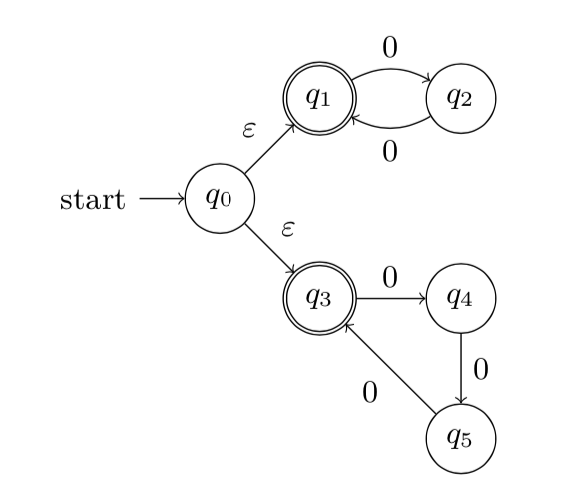
\includegraphics[scale=0.6]{0507182.png}
    \end{center}
    Descrivere il linguaggio e convertirlo in un DFA.
    \item Considerate il linguaggio $L = \{0^n 1^m 0^m : n, m > 0\}$. Questo linguaggio è regolare? Dimostrare formalmente la risposta.
\item Sia L un linguaggio regolare su un alfabeto $\Sigma$ e dimostrate che il seguente linguaggio è regolare: \\ \begin{center}
$suffixes(L) = \{y | xy \in L $ per qualche stringa x $ \in \Sigma ^*\}$ \end{center}
    Intuitivamente, suffixes(L) è il linguaggio di tutti i suffissi delle parole che stanno in L.
    \item Costruire una CFG che genera il linguaggio:\\$L=\{a^nb^mc^k |$ con $n=m $ o $ m=k $ e $ n,m,k\geq0\}$
    \item Convertire l’espressione regolare $(0^*1 + 01^*)^*$ in un DFA.
    \item \begin{enumerate}
    \item Dimostrare che il linguaggio $L = 0^{2n}1^n : n \geq 0$ non è regolare.
    \item Considerate il linguaggio $L = \{0^m1^n : m \neq 2n\}$. Questo linguaggio è regolare? Giustificare formalmente la risposta (la giustificazione non dovrebbe richiedere più di due righe di testo).
    \end{enumerate}
    \item Sia L un linguaggio regolare su un alfabeto $\Sigma$. Supponete che il simbolo $\# \in \Sigma$ e dimostrate che il seguente linguaggio è regolare:
\\\begin{center}$dehash(L) = \{dehash(w) : w \in L\}$\end{center}
    dove dehash(w) è la stringa che si ottiene eliminando tutti i simboli $\#$ da w.
    \item Si consideri la seguente grammatica libera da contesto G: $S \rightarrow iS | iSeS | \epsilon$. Dire e dimostrare che linguaggio accetta e se ambigua. In caso affermativo trovare una grammatica non ambigua che accetti lo stesso linguaggio.
 %   \item Sia $L=\{0^{2n}10^n, n\in\mathbb{N}\}$. Dire se il linguaggio è regolare e, a seconda della risposta (da motivare), definire una CFG o un FA che accetti tale $L$;
   % \item Sia data la CFG:\\$S\rightarrow aB$\\$B\rightarrow Ab|b$\\$A\rightarrow aB|a$\\Definire il suo linguaggio e motivare la propria asserzione;
  % \item Sia $L=\{0^{2n}10^{n^2}, n\in\mathbb{N}\}$. Dire se il linguaggio è regolare e, a seconda della risposta (da motivare), definire una CFG o un FA che accetti tale $L$;
\end{enumerate}
\begin{comment}
\subsection{Soluzioni}
\begin{enumerate}
\item    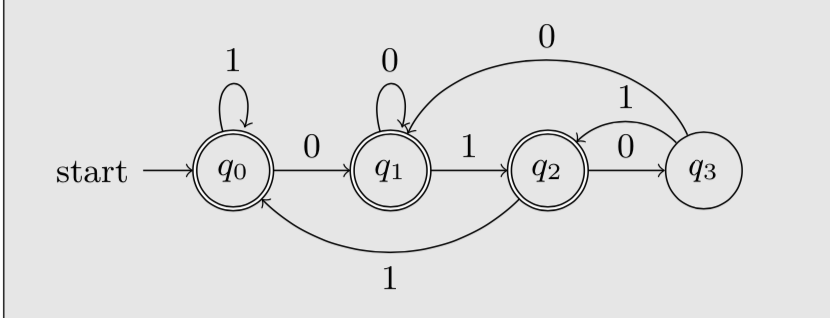
\includegraphics[scale=0.6]{Lez6sol1.png}\\
\item    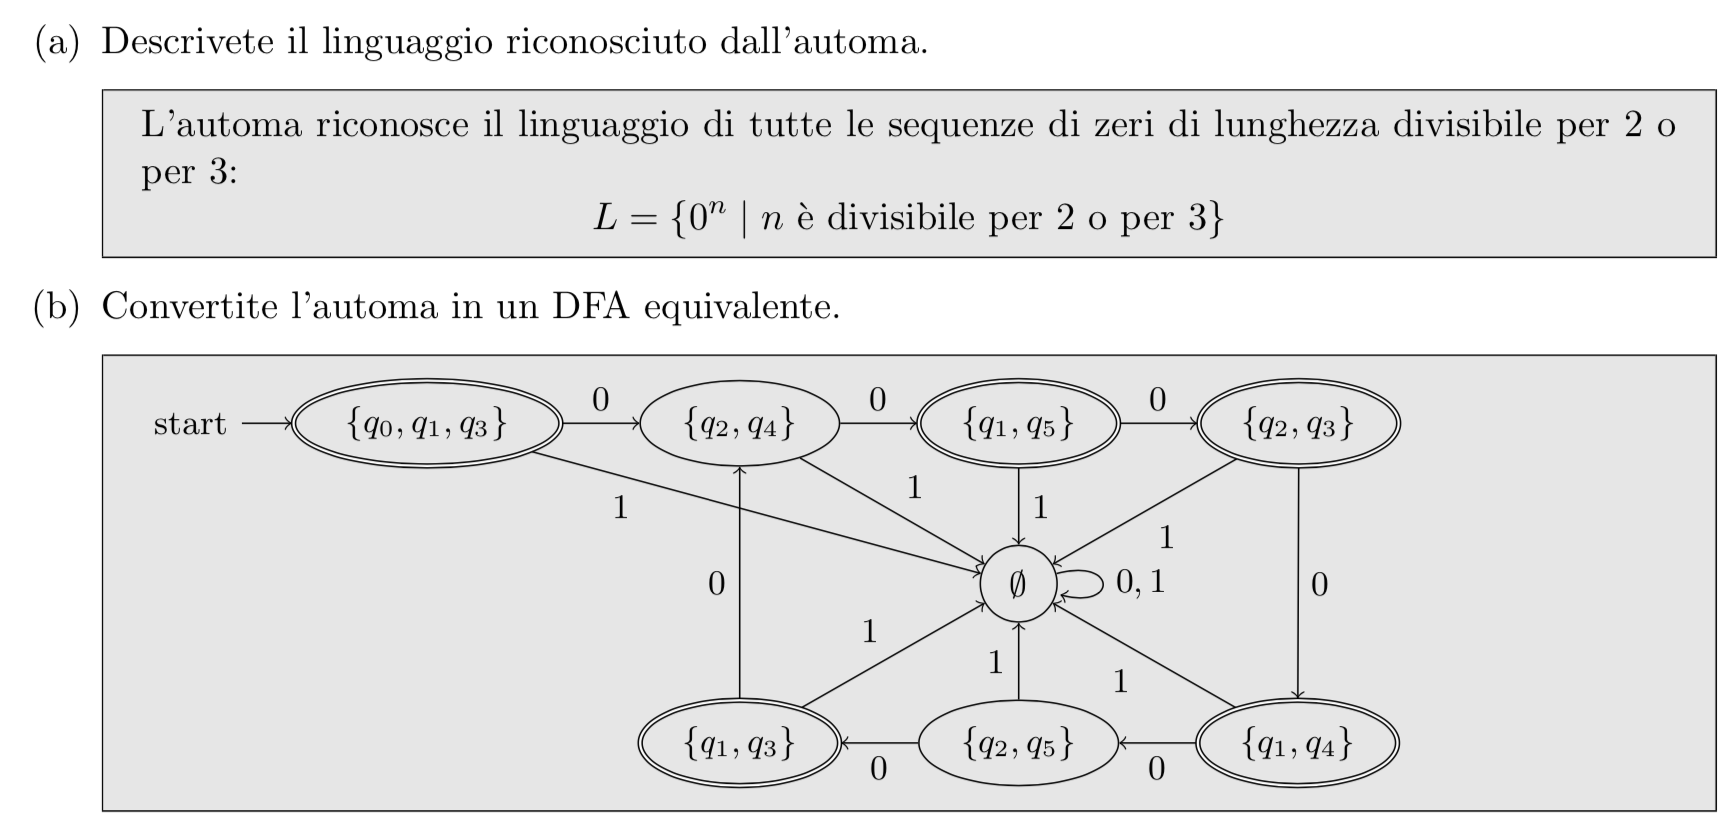
\includegraphics[scale=0.6]{Lez6sol2.png}\\
\item    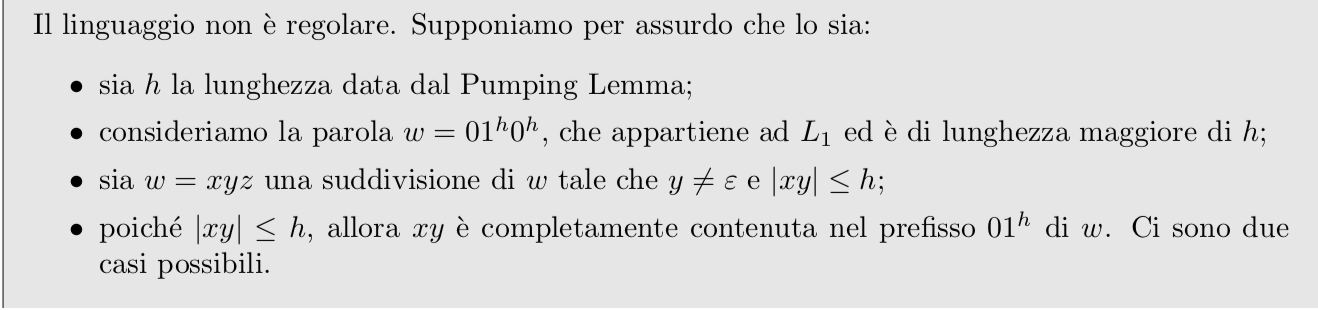
\includegraphics[scale=0.6]{Lez6sol3_1.png}
    \includegraphics[scale=0.6]{lez6sol3_2.png}
\end{enumerate}
\end{comment}
\begin{comment}
Si ha $L(G)=\{a^nb^m|n,m\in\mathbb{N},n+m\geq 1\}=L$. L'asserzione va dimostrata per induzione in entrambi i versi. Una traccia alla dimostrazione è la seguente:
\begin{enumerate}
    \item ("$\Rightarrow$")\\Caso base: 1 derivazione, cioè $S\Rightarrow a$ o $S\Rightarrow b$ entrambe apparteSnenti a $L$.\\Caso induttivo: $S\Rightarrow aS\Rightarrow ^{n}aw'$ o $S\Rightarrow bS\Rightarrow ^{n}bw'$, ma $w' \in L$ per ipotesi induttiva. Aggiungendo una $a$ all'inizio o una $b$ alla fine rimane comunque una stringa in $L$;
    \item ("$\Leftarrow$")\\Caso base: lunghezza 1, cioè $w=a$ o $w=b$. Naturalmente $L(G)$ contiene queste stringhe perché ci sono direttamente le produzioni che lo fanno.\\Caso induttivo: $|w|=n+1$. Allora $w=w'b$ o $w=aw'$. Per ipotesi induttiva $S=>^{*}w'$. Quindi: $S\Rightarrow aS\Rightarrow aw'=w$ o $S\Rightarrow bS\Rightarrow bw'=w \: \Rightarrow w\in L(G)$.
\end{enumerate}
\end{comment}
    % Bibliografia
    %\begin{thebibliography}{9}
        %  Alcune soluzio
    %\end{thebibliography}
    \end{document}